\documentclass[11pt]{article}
\usepackage[utf8]{inputenc}	% Para caracteres en español
\usepackage{amsmath,amsthm,amsfonts,amssymb,amscd}
\usepackage{flexisym}
\usepackage{multirow,booktabs}
\usepackage{fullpage}
\usepackage{lastpage}
\usepackage{enumitem}
\usepackage{fancyhdr}
\usepackage{mathrsfs}
\usepackage{wrapfig}
\usepackage{setspace}
\usepackage[svgnames,table]{xcolor}
% \usepackage{amssymb,mathtools}
\usepackage{cancel}
\usepackage[retainorgcmds]{IEEEtrantools}
\usepackage[margin=3cm]{geometry}
\usepackage{tikz}
\usetikzlibrary{positioning}
\usepackage{amsmath}
\usepackage{mathtools}          %loads amsmath as well
\newlength{\tabcont}
\setlength{\parindent}{0.0in}
\setlength{\parskip}{0.05in}
\usepackage{empheq}
\usepackage{framed}
\usepackage[most]{tcolorbox}
\usepackage{xcolor}
\colorlet{shadecolor}{orange!15}
\parindent 0in
\parskip 12pt
\geometry{margin=1in, headsep=0.25in}
\theoremstyle{definition}
\newtheorem{defn}{Definition}
\newtheorem{reg}{Rule}
\newtheorem{exer}{Exercise}
\newtheorem{sln}{Solution}
\newtheorem{note}{Note}
\setcounter{section}{0}
\title{The Laplace Transform}
\newcommand{\bb}{\mathcal{L}}
\begin{document}

\thispagestyle{empty}
\begin{center}
    \textsc{\LARGE German University in Cairo}\\[1.0cm]
    {\LARGE \bf Laplace Summary}\\ [0.5cm]
    {\large \bf Math301}\\ [0.5cm]
    Fall 2020
\end{center}
\tableofcontents

\section{Basic Definition of Laplace Transform}
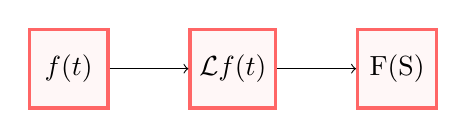
\begin{tikzpicture}[
    squarednode/.style={rectangle, draw=red!60, fill=red!3, very thick, minimum size=10mm},
    ]
    %Nodes
    \node[squarednode]      (maintopic)                              {$f(t)$};
    \node[squarednode]      (rightsquare)       [right=of maintopic] {$\bb{f(t)}$};
    \node[squarednode]      (rightsquare1)       [right=of rightsquare] {F(S)};

    %Lines
    \draw[->] (maintopic.east) -- (rightsquare.west);
    \draw[->] (rightsquare.east) -- (rightsquare1.west);
\end{tikzpicture}
\\
\begin{itemize}
    \item Converts integral equation $\&$ DE's into algebric equations.
    \item  \textsc{Coversion from \textcolor{red}{Time-domain} to \textcolor{red}{Frequency-domain}}
    \item Applications of Laplace Transform: in ODE,PDE, integral equations, etc \dotsc    
\end{itemize}        
\begin{equation}
    F(S) = \bb{f(t)} = \int_0^\infty f(t).e^{-st}dt; \ for\  t\geq0
\end{equation}
\textbf{Improper Integral}

\begin{equation}
    \int_0^\infty f(t)e^{-st} dt = \displaystyle{\lim_{b \to \infty}} \int_0^b f(t).e^{-st} dt
\end{equation}    

\textbf{Note} \\ 

\begin{itemize}
    \item Laplace Transform is applicable to continuous and discontinuous functions.
    \item The Laplace Transform is used if $f(t)$ is given without any integral, if given with interval use \textsc{basic definition}
\end{itemize}

\section{Laplace Transform Properties} 

\subsection{Lineraty of Laplace Transform}

\begin{itemize}
    \item $ \bb{[f(t) \pm g(t)]} = \bb{f(t)} \pm \bb{g(t)}$
    \item $ \bb{[cf(t)]} = c\bb{(f(t))} = cF(S)$ 
\end{itemize}    

\subsection{S- Shifiting property}

\begin{equation}
    \bb{(e^{at}f(t))} = F(S-a)
\end{equation}

\subsection{Laplace Transform of dervatives} 

\begin{itemize}
    \item $ \bb{[f\textprime(t)]} = S\bb(f) - F(0)  $
    \item  $\bb[f\textprime\textprime(t)] = S^2\bb[f] - Sf(0) - f\textprime(0) $    
    \item for \ n \geq 1; \bb[f^{(n)}] = S^{(n)}\bb[f] - S^{(n-1)}f(0) - S^{(n-2)}f\textprime(0) - \dotsc f^{(n-1)}(0)
\end{itemize}

\subsection{Laplace Transform of Integrals}

\begin{equation}
    \bb[\int_0^tf(\tau)d\tau] = \frac{F(S)}{S}
\end{equation}

\subsection{Dervative of Laplace Transform}
\begin{itemize}
    \item $\bb[tf(t)] = -F\textprime(S) $
    \item $\bb[t^2f(t)] = F\textprime \textprime(S)$ 
    \item $\bb[t^nf(t)] = {(-1)}^n \frac{d^n}{dS^n} F(S)$    
\end{itemize}         

\subsection{Integral of Laplace Transform}
\begin{equation}
    \bb[\frac{f(t)}{t}] = \int_S^\infty F(U)dU
\end{equation}    

\subsection{Heaviside function (Unit step Function)} 

\[   
    H(t- a) = 
    \begin{cases}
        0, & \text{$t < a$} \\ 
        1, & \text{$t > a$}
    \end{cases}
\]
\begin{center}
    \includegraphics[scale=0.15]{result.png}
\end{center}


\[   
    H(t) = 
    \begin{cases}
        0, & \text{$t < 0$} \\ 
        1, & \text{$t > 0$}
    \end{cases}
\]
\begin{center}
    \includegraphics[scale=0.15]{result1.png}
\end{center}


\[   
    H(t- b) = 
    \begin{cases}
        0, & \text{$t < b$} \\ 
        1, & \text{$t > b$}
    \end{cases}
\]

\begin{center}
    \includegraphics[scale=0.15]{result3.png}
\end{center}

\subsubsection{Notes}
\begin{itemize}
    \item $H(f(t)) = \square; a< t < b$ 
        \begin{enumerate}
            \item by definition $F(S) = \int_a^b\square e^{-st} dt$
            \item by unit step $f(t) = \square[H(t-a)H(t-b)]$   
        \end{enumerate}

    \item $H(f(t)) = \square; t < b$ 
        \begin{enumerate}
            \item by definition $F(S) = \int_b^\infty \square e^{-st} dt$
            \item by unit step $f(t) = \square[H(t-b)]$   
        \end{enumerate}
\end{itemize}
\subsection{t-shifiting property}
\begin{itemize}
        \item $\bb[H(t-a)] = \frac{1}{s}e^{-as}$
        \item $\bb[f(t-a)H(t-a)]= F(S)e^{-as}$
\end{itemize}
\subsection{Dirac's Delta Function}



\end{document}

